\documentclass[9pt,addpoints]{exam}
\usepackage{enumitem}
\usepackage{amsfonts,amssymb,amsmath, amsthm}
\usepackage{graphicx}
\usepackage{systeme}
\usepackage{pgf,tikz,pgfplots}
\pgfplotsset{compat=1.15}
\usepgfplotslibrary{fillbetween}
\usepackage{mathrsfs}
\usetikzlibrary{arrows}
\usetikzlibrary{calc}
\pagestyle{headandfoot}
%\firstpageheadrule
\runningheader{Homework 2 Solution}{}{Page \thepage\ of \numpages}
\runningheadrule
\author{Aaron GK}
\usepackage{geometry}
\geometry{
	a4paper,
	total={170mm,257mm},
	left=10mm,
	right=10mm,
	bottom=5mm,
	top=5mm,
}
\firstpagefooter{}{}{}
\runningfooter{}{}{}


\begin{document}
	\title{St John Baptist De La Salle Catholic School, Addis Ababa\\
		\large Homework 2 Solution \\
		3rd Quarter}
	\maketitle
	\begin{center}
		\fbox{\fbox{\parbox{6in}{\centering
					Notes, and use of other aids is allowed.  Read all directions carefully and write your answers in the space provided.  To receive full credit, you must show all of your work. \textbf{Cheating or indications of cheating and similar answers will be punished accordingly}. 
		}}}
		\subsubsection*{Information}
		\begin{itemize}
			\item The homework is due on \textbf{Friday}, \textbf{March 3}.
			\item You should Work on it \textbf{in groups} and consult me if you have any questions. Cheating within groups is unacceptable.
			\item For purposes of neatness and simplicity of grading, you should do the homework on an \textbf{A-4 paper}.
		\end{itemize}
	\end{center}
	\begin{center}
		\subsection*{Questions}
	\end{center}
	\begin{questions}
		\question When is the cross product used? How is it different from the dot product? What are the applications of the cross product? \\ \textbf{Answer:} \\ 
		
		Cross product is used in situation in which the product of the vectors results in a vector. It is mainly different from the dot product in that the result in a dot product is always a scalar, whereas a vector product results in a vector. We use the cross product in many situations involving product of vectors giving vectors; it is applicable while finding the directions of many essential vectors such as the force \& torque.
		
		\question Let $\vec{A}=-\hat{i}+2\hat{j}+5\hat{k}$ and $\vec{D}=9\hat{i}-H\hat{j}+5\hat{k}$. For what value(s) of H are the vectors A and D perpendicular? \\ \textbf{Answer:} \\ 
		We know that the dot product of two vectors is 0 when they are perpendicular. If the vectors $\vec{A}$ and $\vec{D}$ are perpendicular, $\vec{A}\cdot\vec{D}=0$ 
		$$\vec{A}\cdot\vec{D}=0$$
		$$(-\hat{i}+2\hat{j}+5\hat{k})\cdot(9\hat{i}-H\hat{j}+5\hat{k})=0$$
		$$-9-2H+25=0\implies-2H=-16$$
		$$H=8$$
		\question After you find the value of H, find $\vec{A}\times\vec{D}$, $|\vec{A}\times\vec{D}|$, and a unit vector perpendicular to both $\vec{A}$ and $\vec{D}$. \\ \textbf{Answer:} \\ 
		$$\vec{A}=(-\hat{i}+2\hat{j}+5\hat{k})\times(9\hat{i}-8\hat{j}+5\hat{k})$$
		To calculate the cross product, we simply can use the matrix method
		\begin{center}
		$\begin{vmatrix}
			\bf \hat{i} & \bf \hat{j} & \bf \hat{k}\\
			-1 & 2 & 5\\
			9 & -8 & 5 
		\end{vmatrix}$	
		\end{center}
		$$\vec{A}\times\vec{D}=\hat{i}(10+40)-\hat{j}(-5-45)+\hat{k}(8-18)$$
		$$\vec{A}\times\vec{D}=50\hat{i}+50\hat{j}-10\hat{k}$$
		$$|\vec{A}\times\vec{D}|=\sqrt{50^2+50^2+(-10)^2}=\sqrt{5100}=10\sqrt{51}$$
		To find a unit vector perpendicular to both $\vec{A}$ and $\vec{D}$, we can just find the unit vector in the direction of $\vec{A}\times\vec{D}$. Let us, for example, name that vector $\hat{n}$;
		$$\hat{n}=\dfrac{\vec{A}\times\vec{D}}{|\vec{A}\times\vec{D}|}=\dfrac{50\hat{i}+50\hat{j}-10\hat{k}}{10\sqrt{51}}=\dfrac{5\hat{i}+5\hat{j}-\hat{k}}{\sqrt{51}}$$
		\question For two vectors $\vec{A} = A_{x}\hat{i} + A_{y}\hat{j} + A_{z}\hat{k}$ and $\vec{B} = B_{x}\hat{i} + B_{y}\hat{j} + B_{z}\hat{k}$, show that $(\vec{A}\times\vec{B})\cdot\vec{B}=0$ \\ \textbf{Answer:} \\ 
		$$\vec{A} \times \vec{B} = (A_{y}B_{z} - A_{z}B_{y})\; \hat{i} + (A_{z}B_{x} - A_{x}B_{z})\; \hat{j} + (A_{x}B_{y} - A_{y}B_{x})\; \hat{k}$$
		$$(\vec{A}\times\vec{B})\cdot\vec{B}$$
		$$((A_{y}B_{z} - A_{z}B_{y})\; \hat{i} + (A_{z}B_{x} - A_{x}B_{z})\; \hat{j} + (A_{x}B_{y} - A_{y}B_{x})\; \hat{k})\cdot(B_x\hat{i}+B_y\hat{j}+B_z\hat{j})$$	
		$$(A_yB_z-A_zB_y)B_x+(A_zB_x-A_xB_z)B_y+(A_xB_y-A_yB_x)B_z$$
		$$(A_yB_zB_x-A_zB_yB_x)+(A_zB_xB_y-A_xB_zB_y)+(A_xB_yB_z-A_yB_xB_z)$$
		We can see that the above terms cancel out to give 0.
		\begin{center}
			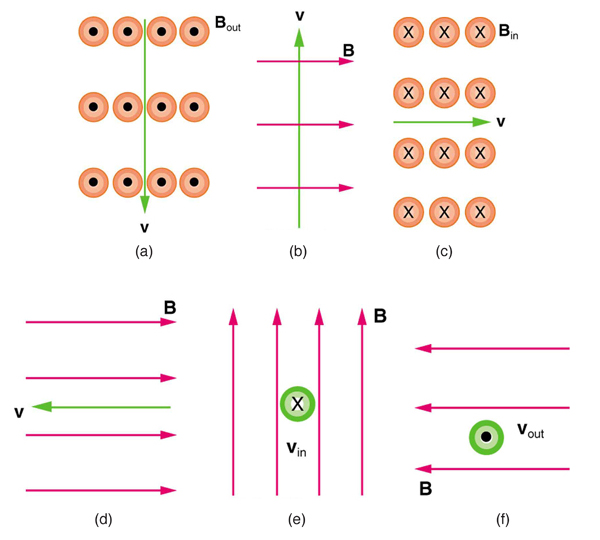
\includegraphics[scale=0.8]{hw_fields_force.jpg}
		\end{center}
		\question For the figure above, find the direction towards which a positive charge would be moving in the various magnetic fields. \\ \textbf{Answer:} \\ 
		\begin{enumerate}[label=(\alph*)]
			\item q$\vec{v}\times\vec{B}\implies-\hat{j}\times\hat{k}=-\hat{i}$: the charge will move to the left.
			\item q$\vec{v}\times\vec{B}\implies\hat{j}\times\hat{i}=-\hat{k}$: the charge will move out of the page.
			\item q$\vec{v}\times\vec{B}\implies\hat{i}\times-\hat{k}=\hat{j}$: the charge will move upwards.
			\item q$\vec{v}\times\vec{B}\implies-\hat{i}\times\hat{i}=0$: the charge \textbf{will keep moving }to the left.
			\item q$\vec{v}\times\vec{B}\implies-\hat{k}\times\hat{j}=\hat{i}$: the charge will move to the right.
			\item q$\vec{v}\times\vec{B}\implies\hat{k}\times-\hat{i}=-\hat{j}$: the charge will move downwards.
		\end{enumerate}
		\question A charged particle of mass twice that of an electron and a charge of -3.2$\times10^{-19}$C is moving about a circular trajectory of radius 20cm in a uniform $3.5\times10^3$G magnetic field that is perpendicular to the velocity of the charge. What is the velocity of the charge? \\ \textbf{Answer:} \\ 
		$$qvB\sin\theta=\dfrac{mv^2}{r}$$
		$$v=\dfrac{qBr\sin\theta}{m}$$
		$$v=\dfrac{3.2\times10^{-19}C\times3.5\times10^{-1}T\times0.2m}{2\times9.11\times10^{-31}kg}$$
		\question An electron moving at a speed of 0.7$c$ through a magnetic field of 2.0T experiences a magnetic force of $2.2\times10^{-14}$N. What is the angle between the electron's velocity and the magnetic field? \\ \textbf{Answer:} \\ 
		$$F=qvB\sin\theta$$
		$$\sin\theta=\dfrac{F}{qvB}$$
		$$\sin\theta=\dfrac{2.2\times10^{-14}N}{1.6\times10^{-19}C\times0.7\times3\times10^8m/s\times2.0T}=\dfrac{2.2\times10^{-14}N}{3.2\times2.1\times10^{-11}N}=\dfrac{2.2}{3.2\times2.1}\times10^{-3}$$
		$$\theta=\sin^{-1}\left(\dfrac{2.2}{3.2\times2.1}\times10^{-3}\right)$$
		\subsection*{Advanced Problems}
		\question A uniform magnetic field of magnitude 1.2 T is directed along the negative y - axis. An electron moving at a speed of 0.2$c$ makes an angle of 60$^0$ with the y - axis. Answer the following questions.
		\begin{enumerate}[label=(\Roman*)]
			\item What is the expected trajectory of the electron? \\ \textbf{Answer:} \\ 
			The expected trajectory is a helix. That is because the perpendicular component of the velocity will make the electron travel about a circle while the parallel component keeps the electron in its original path. The superposition of the two motions results in a helical trajectory.
			\item Calculate the radius \& pitch of the trajectory. \\ \textbf{Answer:} \\ 
			$$r=\dfrac{mv}{qB\sin\theta}$$
			$$r=\dfrac{9.11\times10^{-31}kg\times0.2\times3\times10^8m/s}{1.6\times10^{-19}C\times1.2T\times\sin60^0}$$
			To calculate the pitch, first let's look at what it is. The pitch is the distance traveled parallel to the magnetic field B in one revolution. Thus,
			$$p=v_{\parallel}T\text{ where T is the time needed to complete a revolution}$$ 
			To calculate the pitch, we first need to calculate the time it takes to complete a revolution.
			$$v_{\perp}=\dfrac{2\pi R}{T}$$
			$$T=\dfrac{2\pi R}{v_{\perp}}$$
			Then, we can calculate the pitch as follows:
			$$p=v_{\parallel}(\dfrac{2\pi R}{v_{\perp}})$$
			$$p=v\cos\theta(\dfrac{2\pi R}{v\sin\theta})=\cos\theta(\dfrac{2\pi R}{\sin\theta})$$
			$$p=(\dfrac{2\pi R}{\tan\theta})$$
			$$p=\dfrac{2\pi\times\dfrac{9.11\times10^{-31}kg\times0.2\times3\times10^8m/s}{1.6\times10^{-19}C\times1.2T\times\sin60^0}}{\tan 60^0}$$
		\end{enumerate}
	\end{questions}		
\end{document}